%---------------
%╔═╗╔═╗╔╦╗╦  ╦╔═╗
%╚═╗║╣    ║  ║  ║╠═╝
%╚═╝╚═╝  ╩  ╚═╝╩  
%---------------

% language setup
\newcommand{\docLanguage}{ngerman}
%\newcommand{\docLanguage}{english}

% DOCUMENT SETUP
\documentclass[12pt, oneside, a4paper, \docLanguage]{report}
\usepackage[left=3cm, 
			right=2.5cm, 
			top=2.5cm, 
			bottom=2.5cm, 
			includehead, 
			includefoot]{geometry}

% line spacing
\usepackage{setspace}
\setstretch{1,25} % 15/12 --> 1.25

% encoding setup
% T1 font encoding for languages that use a latin alphabet
\usepackage[T1]{fontenc} 

% enhanced input encoding handling - utf8 for äÄüÜöÖß...
\usepackage[utf8]{inputenc}

%de­fines Adobe Times Ro­man as de­fault text font
\usepackage{mathptmx}
\usepackage{times} % needed for acronym package

%PDF linking package
\usepackage[hidelinks]{hyperref}


% Language Setup
\usepackage[\docLanguage]{babel}
% after babel - set chapter string
\AtBeginDocument{\renewcommand{\chaptername}{}}

% language specific bibliography style
\usepackage[numbers, square]{natbib}
%\setcitestyle{square,aysep={},yysep={;}}
\usepackage[fixlanguage]{babelbib}
\selectbiblanguage{\docLanguage}
% bliographystyle setup
% babel specific: babplain, babplai3, babalpha, babunsrt, bababbrv, bababbr3
\bibliographystyle{babunsrt}


% enumeration
\usepackage{enumitem}
% tabular extension tabularx
\usepackage{tabularx}

% math packages
\usepackage{amsmath}
\usepackage{nicefrac}
\usepackage{amsthm}
\usepackage{amsbsy}
\usepackage{amssymb}
\usepackage{amsfonts}
%\usepackage{MnSymbol}


%special characters
\usepackage{amssymb}
\usepackage{upgreek,textgreek}

% acronym package
\usepackage[printonlyused, footnote]{acronym}

% breakable text in \seqsplit{}
\usepackage{seqsplit}

% \textmu
\usepackage{textcomp}

% package provides a way to compile sections of a document using the same preamble as the main document
\usepackage{subfiles}

% driver-independent color extension - used by listings,tabularx
\usepackage[usenames,dvipsnames,table,xcdraw]{xcolor}

% -- SYNTAX HIGHLIGHTING --
\usepackage{listings}
%% bash command line Syntax Highlighting
\lstdefinestyle{BASH_CMD}{ 
  columns=fullflexible,            % copy pasteable listings
  language=bash,
  basicstyle=\small\sffamily,
  basicstyle   = \small \ttfamily,
  keywordstyle = [1]\small \ttfamily,
  keywordstyle = [2]\small \ttfamily,
  commentstyle = \small \ttfamily,
  numbers=none,
  captionpos=b, 
  breaklines=true,
  numberstyle=\tiny,
  numbersep=3pt,
  frame=tlrb,
  columns=fullflexible,
  backgroundcolor=\color{white!20},
  linewidth=\linewidth,
  literate=                        % replace in code
     {Ö}{{\"O}}1 
     {Ä}{{\"A}}1 
     {Ü}{{\"U}}1 
     {ß}{{\ss}}2 
     {ü}{{\"u}}1 
     {ä}{{\"a}}1 
     {ö}{{\"o}}1 
     {â}{{\^{a}}}1 
     {Â}{{\^{A}}}1 
     {ç}{{\c{c}}}1 
     {Ç}{{\c{C}}}1 
     {ğ}{{\u{g}}}1 
     {Ğ}{{\u{G}}}1 
     {ı}{{\i}}1 
     {İ}{{\.{I}}}1 
     {ş}{{\c{s}}}1 
     {Ş}{{\c{S}}}1 
}
 % adds style BASH_CMD
%% Matlab Syntax Highlighting
\colorlet{keyword}{blue!100!black!80}
\colorlet{STD}{Lavender}
\colorlet{comment}{green!90!black!90}
\definecolor{mygreen}{rgb}{0,0.6,0}
\definecolor{mygray}{rgb}{0.5,0.5,0.5}
\definecolor{mymauve}{rgb}{0.58,0,0.82}


\lstdefinestyle{BASH_SCRIPT}{ 
  language     = bash,
  basicstyle   = \footnotesize \ttfamily,
  keywordstyle = [1]\color{keyword}\bfseries,
  keywordstyle = [2]\color{STD}\bfseries,
  commentstyle = \color{mygreen}\itshape,
  backgroundcolor=\color{white},   % choose the background color; you must add \usepackage{color} 
  columns=fullflexible,            % copy pasteable listings
                                   % or \usepackage{xcolor}
  basicstyle=\footnotesize,        % the size of the fonts that are used for the code
  breakatwhitespace=false,         % sets if automatic breaks should only happen at whitespace
  breaklines=true,                 % sets automatic line breaking
  captionpos=b,                    % sets the caption-position to bottom
  extendedchars=true,              % lets you use non-ASCII characters; for 8-bits encodings only,
                                   % does not work with UTF-8
  frame=single,                    % adds a frame around the code
  keepspaces=true,                 % keeps spaces in text, useful for keeping indentation of code
                                   % (possibly needs columns=flexible)
  numbers=left,                    % where to put the line-numbers; possible values are 
                                   % (none, left, right)
  numbersep=5pt,                   % how far the line-numbers are from the code
  numberstyle=\tiny\color{mygray}, % the style that is used for the line-numbers
  rulecolor=\color{black},         % if not set, the frame-color may be changed on line-breaks
                                   % within not-black text (e.g. comments (green here))
  showspaces=false,                % show spaces everywhere adding particular underscores; it
  	                               % overrides 'showstringspaces'
  showstringspaces=false,          % underline spaces within strings only
  showtabs=false,                  % show tabs within strings adding particular underscores
  stepnumber=1,                    % the step between two line-numbers. If it's 1, each line 
                                   % will be numbered
  stringstyle=\color{mymauve},     % string literal style
  tabsize=2,                       % sets default tabsize to 2 spaces
  title=\lstname,                  % set title name
  literate=                        % replace in code
     {Ö}{{\"O}}1 
     {Ä}{{\"A}}1 
     {Ü}{{\"U}}1 
     {ß}{{\ss}}2 
     {ü}{{\"u}}1 
     {ä}{{\"a}}1 
     {ö}{{\"o}}1 
     {â}{{\^{a}}}1 
     {Â}{{\^{A}}}1 
     {ç}{{\c{c}}}1 
     {Ç}{{\c{C}}}1 
     {ğ}{{\u{g}}}1 
     {Ğ}{{\u{G}}}1 
     {ı}{{\i}}1 
     {İ}{{\.{I}}}1 
     {ş}{{\c{s}}}1 
     {Ş}{{\c{S}}}1 
} % adds style BASH_SCRIPT
% Matlab Syntax Highlighting
\colorlet{keyword}{blue!100!black!80}
\colorlet{STD}{red}
\colorlet{comment}{green!90!black!90}
\definecolor{mygreen}{rgb}{0,0.6,0}
\definecolor{mygray}{rgb}{0.5,0.5,0.5}
\definecolor{mymauve}{rgb}{0.58,0,0.82}


\lstdefinestyle{LATEX}{ 
  language     = [LaTeX]{TeX},
  basicstyle   = \footnotesize \ttfamily,
  keywordstyle = [1]\color{keyword}\bfseries,
  keywordstyle = [2]\color{comment}\bfseries,
  commentstyle = \color{mygray}\itshape,
  %backgroundcolor=\color{white},   % choose the background color; you must add \usepackage{color} 
                                   % or \usepackage{xcolor}
  basicstyle=\footnotesize,        		   % the size of the fonts that are used for the code
  breakatwhitespace=false,         % sets if automatic breaks should only happen at whitespace
  columns=fullflexible,            % copy pasteable listings
  breaklines=true,                 % sets automatic line breaking
  captionpos=c,                    % sets the caption-position to bottom
  extendedchars=true,              % lets you use non-ASCII characters; for 8-bits encodings only,
                                   % does not work with UTF-8
  frame=single,                    % adds a frame around the code
  keepspaces=true,                 % keeps spaces in text, useful for keeping indentation of code
                                   % (possibly needs columns=flexible)
  numbers=left,                    % where to put the line-numbers; possible values are 
                                   % (none, left, right)
  numbersep=4pt,                   % how far the line-numbers are from the code
  numberstyle=\tiny\color{mygray}, % the style that is used for the line-numbers
  rulecolor=\color{black},         % if not set, the frame-color may be changed on line-breaks
                                   % within not-black text (e.g. comments (green here))
  showspaces=false,                % show spaces everywhere adding particular underscores; it
  	                               % overrides 'showstringspaces'
  showstringspaces=false,          % underline spaces within strings only
  showtabs=false,                  % show tabs within strings adding particular underscores
  stepnumber=1,                    % the step between two line-numbers. If it's 1, each line 
                                   % will be numbered
  stringstyle=\color{mymauve},     % string literal style
  tabsize=2,                       % sets default tabsize to 2 spaces
  title=\lstname,                  % set title name
  literate=                        % replace in code
     {Ö}{{\"O}}1 
     {Ä}{{\"A}}1 
     {Ü}{{\"U}}1 
     {ß}{{\ss}}2 
     {ü}{{\"u}}1 
     {ä}{{\"a}}1 
     {ö}{{\"o}}1 
     {â}{{\^{a}}}1 
     {Â}{{\^{A}}}1 
     {ç}{{\c{c}}}1 
     {Ç}{{\c{C}}}1 
     {ğ}{{\u{g}}}1 
     {Ğ}{{\u{G}}}1 
     {ı}{{\i}}1 
     {İ}{{\.{I}}}1 
     {ş}{{\c{s}}}1 
     {Ş}{{\c{S}}}1 
} % adds style LATEX
%% Matlab Syntax Highlighting
\colorlet{keyword}{blue!100!black!80}
\colorlet{STD}{Lavender}
\colorlet{comment}{green!90!black!90}
\definecolor{mygreen}{rgb}{0,0.6,0}
\definecolor{mygray}{rgb}{0.5,0.5,0.5}
\definecolor{mymauve}{rgb}{0.58,0,0.82}


\lstdefinestyle{MATLAB}{ 
  language     = Matlab,
  basicstyle   = \footnotesize \ttfamily,
  keywordstyle = [1]\color{keyword}\bfseries,
  keywordstyle = [2]\color{STD}\bfseries,
  commentstyle = \color{mygreen}\itshape,
  backgroundcolor=\color{white},   % choose the background color; you must add \usepackage{color} 
                                   % or \usepackage{xcolor}
  basicstyle=\footnotesize,        % the size of the fonts that are used for the code
  breakatwhitespace=false,         % sets if automatic breaks should only happen at whitespace
  columns=fullflexible,            % copy pasteable listings
  breaklines=false,                % sets automatic line breaking
  captionpos=c,                    % sets the caption-position to bottom
  extendedchars=true,              % lets you use non-ASCII characters; for 8-bits encodings only,
                                   % does not work with UTF-8
  frame=single,                    % adds a frame around the code
  keepspaces=true,                 % keeps spaces in text, useful for keeping indentation of code
                                   % (possibly needs columns=flexible)
  numbers=left,                    % where to put the line-numbers; possible values are 
                                   % (none, left, right)
  numbersep=5pt,                   % how far the line-numbers are from the code
  numberstyle=\tiny\color{mygray}, % the style that is used for the line-numbers
  rulecolor=\color{black},         % if not set, the frame-color may be changed on line-breaks
                                   % within not-black text (e.g. comments (green here))
  showspaces=false,                % show spaces everywhere adding particular underscores; it
  	                               % overrides 'showstringspaces'
  showstringspaces=false,          % underline spaces within strings only
  showtabs=false,                  % show tabs within strings adding particular underscores
  stepnumber=1,                    % the step between two line-numbers. If it's 1, each line 
                                   % will be numbered
  stringstyle=\color{mymauve},     % string literal style
  tabsize=2,                       % sets default tabsize to 2 spaces
  title=\lstname,                  % set title name
  literate=                        % replace in code
     {Ö}{{\"O}}1 
     {Ä}{{\"A}}1 
     {Ü}{{\"U}}1 
     {ß}{{\ss}}2 
     {ü}{{\"u}}1 
     {ä}{{\"a}}1 
     {ö}{{\"o}}1 
     {â}{{\^{a}}}1 
     {Â}{{\^{A}}}1 
     {ç}{{\c{c}}}1 
     {Ç}{{\c{C}}}1 
     {ğ}{{\u{g}}}1 
     {Ğ}{{\u{G}}}1 
     {ı}{{\i}}1 
     {İ}{{\.{I}}}1 
     {ş}{{\c{s}}}1 
     {Ş}{{\c{S}}}1 
} % adds style MATLAB
% Matlab Syntax Highlighting
\colorlet{keyword}{blue!100!black!80}
\colorlet{STD}{Lavender}
\colorlet{comment}{green!90!black!90}
\definecolor{mygreen}{rgb}{0,0.6,0}
\definecolor{mygray}{rgb}{0.5,0.5,0.5}
\definecolor{mymauve}{rgb}{0.58,0,0.82}


\lstdefinestyle{PYTHON}{ 
  language     = Python,
  basicstyle   = \footnotesize \ttfamily,
  keywordstyle = [1]\color{keyword}\bfseries,
  keywordstyle = [2]\color{STD}\bfseries,
  commentstyle = \color{mygreen}\itshape,
  backgroundcolor=\color{white},   % choose the background color; you must add \usepackage{color} 
                                   % or \usepackage{xcolor}
  basicstyle=\footnotesize,        % the size of the fonts that are used for the code
  columns=fullflexible,            % copy pasteable listings
  breakatwhitespace=false,         % sets if automatic breaks should only happen at whitespace
  breaklines=false,                % sets automatic line breaking
  captionpos=c,                    % sets the caption-position to bottom
  extendedchars=true,              % lets you use non-ASCII characters; for 8-bits encodings only,
                                   % does not work with UTF-8
  frame=single,                    % adds a frame around the code
  keepspaces=true,                 % keeps spaces in text, useful for keeping indentation of code
                                   % (possibly needs columns=flexible)
  numbers=left,                    % where to put the line-numbers; possible values are 
                                   % (none, left, right)
  numbersep=5pt,                   % how far the line-numbers are from the code
  numberstyle=\tiny\color{mygray}, % the style that is used for the line-numbers
  rulecolor=\color{black},         % if not set, the frame-color may be changed on line-breaks
                                   % within not-black text (e.g. comments (green here))
  showspaces=false,                % show spaces everywhere adding particular underscores; it
  	                               % overrides 'showstringspaces'
  showstringspaces=false,          % underline spaces within strings only
  showtabs=false,                  % show tabs within strings adding particular underscores
  stepnumber=1,                    % the step between two line-numbers. If it's 1, each line 
                                   % will be numbered
  stringstyle=\color{mymauve},     % string literal style
  tabsize=2,                       % sets default tabsize to 2 spaces
  title=\lstname,                  % set title name
  literate=                        % replace in code
     {Ö}{{\"O}}1 
     {Ä}{{\"A}}1 
     {Ü}{{\"U}}1 
     {ß}{{\ss}}2 
     {ü}{{\"u}}1 
     {ä}{{\"a}}1 
     {ö}{{\"o}}1 
     {â}{{\^{a}}}1 
     {Â}{{\^{A}}}1 
     {ç}{{\c{c}}}1 
     {Ç}{{\c{C}}}1 
     {ğ}{{\u{g}}}1 
     {Ğ}{{\u{G}}}1 
     {ı}{{\i}}1 
     {İ}{{\.{I}}}1 
     {ş}{{\c{s}}}1 
     {Ş}{{\c{S}}}1 
} % adds style PYTHON
%% Matlab Syntax Highlighting
\colorlet{keyword}{blue!100!black!80}
\colorlet{STD}{Lavender}
\colorlet{comment}{green!90!black!90}
\definecolor{mygreen}{rgb}{0,0.6,0}
\definecolor{mygray}{rgb}{0.5,0.5,0.5}
\definecolor{mymauve}{rgb}{0.58,0,0.82}


\lstdefinestyle{CPP}{ 
  language     = C++,
  basicstyle   = \footnotesize \ttfamily,
  keywordstyle = [1]\color{keyword}\bfseries,
  keywordstyle = [2]\color{STD}\bfseries,
  commentstyle = \color{mygreen}\itshape,
  backgroundcolor=\color{white},   % choose the background color; you must add \usepackage{color} 
                                   % or \usepackage{xcolor}
  columns=fullflexible,            % copy pasteable listings
  basicstyle=\footnotesize,        % the size of the fonts that are used for the code
  breakatwhitespace=false,         % sets if automatic breaks should only happen at whitespace
  breaklines=false,                % sets automatic line breaking
  captionpos=c,                    % sets the caption-position to bottom
  extendedchars=true,              % lets you use non-ASCII characters; for 8-bits encodings only,
                                   % does not work with UTF-8
  frame=single,                    % adds a frame around the code
  keepspaces=true,                 % keeps spaces in text, useful for keeping indentation of code
                                   % (possibly needs columns=flexible)
  numbers=left,                    % where to put the line-numbers; possible values are 
                                   % (none, left, right)
  numbersep=5pt,                   % how far the line-numbers are from the code
  numberstyle=\tiny\color{mygray}, % the style that is used for the line-numbers
  rulecolor=\color{black},         % if not set, the frame-color may be changed on line-breaks
                                   % within not-black text (e.g. comments (green here))
  showspaces=false,                % show spaces everywhere adding particular underscores; it
  	                               % overrides 'showstringspaces'
  showstringspaces=false,          % underline spaces within strings only
  showtabs=false,                  % show tabs within strings adding particular underscores
  stepnumber=1,                    % the step between two line-numbers. If it's 1, each line 
                                   % will be numbered
  stringstyle=\color{mymauve},     % string literal style
  tabsize=2,                       % sets default tabsize to 2 spaces
  title=\lstname,                  % set title name
  literate=                        % replace in code
     {Ö}{{\"O}}1 
     {Ä}{{\"A}}1 
     {Ü}{{\"U}}1 
     {ß}{{\ss}}2 
     {ü}{{\"u}}1 
     {ä}{{\"a}}1 
     {ö}{{\"o}}1 
     {â}{{\^{a}}}1 
     {Â}{{\^{A}}}1 
     {ç}{{\c{c}}}1 
     {Ç}{{\c{C}}}1 
     {ğ}{{\u{g}}}1 
     {Ğ}{{\u{G}}}1 
     {ı}{{\i}}1 
     {İ}{{\.{I}}}1 
     {ş}{{\c{s}}}1 
     {Ş}{{\c{S}}}1 
} % adds style CPP
%% Matlab Syntax Highlighting
\colorlet{keyword}{blue!100!black!80}
\colorlet{STD}{Lavender}
\colorlet{comment}{green!90!black!90}
\definecolor{mygreen}{rgb}{0,0.6,0}
\definecolor{mygray}{rgb}{0.5,0.5,0.5}
\definecolor{mymauve}{rgb}{0.58,0,0.82}


\lstdefinestyle{C}{ 
  language     = C,
  basicstyle   = \footnotesize \ttfamily,
  keywordstyle = [1]\color{keyword}\bfseries,
  keywordstyle = [2]\color{STD}\bfseries,
  commentstyle = \color{mygreen}\itshape,
  backgroundcolor=\color{white},   % choose the background color; you must add \usepackage{color} 
  columns=fullflexible,            % copy pasteable listings
                                   % or \usepackage{xcolor}
  basicstyle=\footnotesize,        % the size of the fonts that are used for the code
  breakatwhitespace=false,         % sets if automatic breaks should only happen at whitespace
  breaklines=false,                % sets automatic line breaking
  captionpos=c,                    % sets the caption-position to bottom
  extendedchars=true,              % lets you use non-ASCII characters; for 8-bits encodings only,
                                   % does not work with UTF-8
  frame=single,                    % adds a frame around the code
  keepspaces=true,                 % keeps spaces in text, useful for keeping indentation of code
                                   % (possibly needs columns=flexible)
  numbers=left,                    % where to put the line-numbers; possible values are 
                                   % (none, left, right)
  numbersep=5pt,                   % how far the line-numbers are from the code
  numberstyle=\tiny\color{mygray}, % the style that is used for the line-numbers
  rulecolor=\color{black},         % if not set, the frame-color may be changed on line-breaks
                                   % within not-black text (e.g. comments (green here))
  showspaces=false,                % show spaces everywhere adding particular underscores; it
  	                               % overrides 'showstringspaces'
  showstringspaces=false,          % underline spaces within strings only
  showtabs=false,                  % show tabs within strings adding particular underscores
  stepnumber=1,                    % the step between two line-numbers. If it's 1, each line 
                                   % will be numbered
  stringstyle=\color{mymauve},     % string literal style
  tabsize=2,                       % sets default tabsize to 2 spaces
  title=\lstname,                  % set title name
  literate=                        % replace in code
     {Ö}{{\"O}}1 
     {Ä}{{\"A}}1 
     {Ü}{{\"U}}1 
     {ß}{{\ss}}2 
     {ü}{{\"u}}1 
     {ä}{{\"a}}1 
     {ö}{{\"o}}1 
     {â}{{\^{a}}}1 
     {Â}{{\^{A}}}1 
     {ç}{{\c{c}}}1 
     {Ç}{{\c{C}}}1 
     {ğ}{{\u{g}}}1 
     {Ğ}{{\u{G}}}1 
     {ı}{{\i}}1 
     {İ}{{\.{I}}}1 
     {ş}{{\c{s}}}1 
     {Ş}{{\c{S}}}1 
} % adds style C
%% JSON Syntax Highlighting
\colorlet{keyword}{blue!100!black!80}
\colorlet{STD}{Lavender}
\colorlet{comment}{green!90!black!90}
\definecolor{mygreen}{rgb}{0,0.6,0}
\definecolor{mygray}{rgb}{0.5,0.5,0.5}
\definecolor{mymauve}{rgb}{0.58,0,0.82}

\newcommand\JSONnumbervaluestyle{\color{blue}}
\newcommand\JSONstringvaluestyle{\color{red}}

\newif\ifcolonfoundonthisline

\makeatletter

\lstdefinelanguage{json}
{
  showstringspaces    = false,
  keywords            = {false,true},
  alsoletter          = 0123456789.,
  morestring          = [s]{"}{"},
  morestring          = [s]{'}{'},
  stringstyle         = \ifcolonfoundonthisline\JSONstringvaluestyle\fi,
  MoreSelectCharTable =%
    \lst@DefSaveDef{`:}\colon@json{\processColon@json},
  basicstyle          = \ttfamily,
  keywordstyle        = \ttfamily\bfseries,
}

% flip the switch if a colon is found in Pmode
\newcommand\processColon@json{
  \colon@json%
  \ifnum\lst@mode=\lst@Pmode%
    \global\colonfoundonthislinetrue%
  \fi
}

\lst@AddToHook{Output}{%
  \ifcolonfoundonthisline%
    \ifnum\lst@mode=\lst@Pmode%
      \def\lst@thestyle{\JSONnumbervaluestyle}%
    \fi
  \fi
  %override by keyword style if a keyword is detected!
  \lsthk@DetectKeywords% 
}

% reset the switch at the end of line
\lst@AddToHook{EOL}%
  {\global\colonfoundonthislinefalse}

\makeatother



\lstdefinestyle{JSON}{ 
  language     = json,
  basicstyle   = \footnotesize \ttfamily,
  keywordstyle = [1]\color{keyword}\bfseries,
  keywordstyle = [2]\color{STD}\bfseries,
  commentstyle = \color{mygreen}\itshape,
  backgroundcolor=\color{white},   % choose the background color; you must add \usepackage{color} 
                                   % or \usepackage{xcolor}
  basicstyle=\footnotesize,        % the size of the fonts that are used for the code
  columns=fullflexible,            % copy pasteable listings
  breakatwhitespace=false,         % sets if automatic breaks should only happen at whitespace
  breaklines=false,                % sets automatic line breaking
  captionpos=c,                    % sets the caption-position to bottom
  extendedchars=true,              % lets you use non-ASCII characters; for 8-bits encodings only,
                                   % does not work with UTF-8
  frame=single,                    % adds a frame around the code
  keepspaces=true,                 % keeps spaces in text, useful for keeping indentation of code
                                   % (possibly needs columns=flexible)
  numbers=left,                    % where to put the line-numbers; possible values are 
                                   % (none, left, right)
  numbersep=5pt,                   % how far the line-numbers are from the code
  numberstyle=\tiny\color{mygray}, % the style that is used for the line-numbers
  rulecolor=\color{black},         % if not set, the frame-color may be changed on line-breaks
                                   % within not-black text (e.g. comments (green here))
  showspaces=false,                % show spaces everywhere adding particular underscores; it
  	                               % overrides 'showstringspaces'
  showstringspaces=false,          % underline spaces within strings only
  showtabs=false,                  % show tabs within strings adding particular underscores
  stepnumber=1,                    % the step between two line-numbers. If it's 1, each line 
                                   % will be numbered
  stringstyle=\color{mymauve},     % string literal style
  tabsize=2,                       % sets default tabsize to 2 spaces
  title=\lstname,                  % set title name
  literate=                        % replace in code
     {Ö}{{\"O}}1 
     {Ä}{{\"A}}1 
     {Ü}{{\"U}}1 
     {ß}{{\ss}}2 
     {ü}{{\"u}}1 
     {ä}{{\"a}}1 
     {ö}{{\"o}}1 
     {â}{{\^{a}}}1 
     {Â}{{\^{A}}}1 
     {ç}{{\c{c}}}1 
     {Ç}{{\c{C}}}1 
     {ğ}{{\u{g}}}1 
     {Ğ}{{\u{G}}}1 
     {ı}{{\i}}1 
     {İ}{{\.{I}}}1 
     {ş}{{\c{s}}}1 
     {Ş}{{\c{S}}}1 
} % adds style JSON

% HEADLINE CFG
\usepackage{fancyhdr} % Headers and footers
\usepackage{lastpage}
\usepackage{ifthen}
\setlength{\headheight}{1.5cm}
%\pagestyle{fancy} % All pages have headers and footers
% override plain page style for \part, \chapter or 
% \maketitle, which implicit specifies plain page style
\fancypagestyle{plain} 
{
	\fancyhead[L]{}
	\fancyhead[C]{}
	\fancyhead[R]{}
	\fancyfoot[L]{}
	\fancyfoot[C]{\thepage}
	\fancyfoot[R]{}
}
% set list pagestyle
\fancypagestyle{preface} 
{
	\fancyhead[L]{}
	\fancyhead[C]{}
	\fancyhead[R]{}
	\fancyfoot[L]{}
	\fancyfoot[C]{\thepage}
	\fancyfoot[R]{}
}
% set default pagestyle
\fancypagestyle{default} 
{
	\fancyhead{} % Blank out the default header
	\fancyfoot{} % Blank out the default footer
	\fancyhead[L]{}
	\fancyhead[C]{}
	\fancyhead[R]{}
	\fancyfoot[L]{}
	\fancyfoot[C]{\thepage}
	\fancyfoot[R]{}
}
%\fancypagestyle{default} 
{
\fancyhead[L]{\ifthenelse{\isodd{\value{page}}}{\arabic{chapter} \rightmark}{}}
\fancyhead[R]{\thepage}
}

\renewcommand{\chaptermark}[1]{\markright{#1}{}}
\renewcommand{\sectionmark}[1]{\markright{#1}{}}
\renewcommand{\headrulewidth}{0pt}
\renewcommand{\footrulewidth}{0pt}

% PICTURE CFG 
\usepackage{verbatim}
\usepackage{graphicx}
\usepackage{epstopdf}
\usepackage{caption}
\usepackage[list=true,listformat=simple]{subcaption}
% floating prevention packages
\usepackage{float}    % used with [H] positioning parameter
\usepackage{placeins} % \FloatBarrier 
% tikz packages
\usepackage{tikz}
\usepackage{standalone}
\usepackage{pgfplots}


% include only specified tex files - uncommend here
\includeonly{preface/cover,
             preface/abstract,
             preface/tableofcontents,
             preface/listoffigures,
             preface/listoftables,
             preface/lstlistoflistings,
             appendix/bibliography}

%-------------------
%╔═╗╔╦╗╦═╗╦ ╔╗╔╔═╗╔═╗
%╚═╗  ║  ╠╦╝║ ║║║║ ╦ ╚═╗
%╚═╝  ╩  ╩╚═╩ ╝╚╝╚═╝╚═╝
%-------------------
\newcommand{\strLecture}{Signale, Systeme und Sensoren}
\newcommand{\strDate}{\today}
\newcommand{\strAuthorA}{Kiattipoom Pensuwan}
\newcommand{\strAuthorB}{Thanh Son Dang}
%\newcommand{\strAuthorC}{C. Author}
\newcommand{\strAuthorAEmail}{ki851pen@htwg-konstanz.de}
\newcommand{\strAuthorBEmail}{th851dan@htwg-konstanz.de}
%\newcommand{\strAuthorCEmail}{cauthor@htwg-konstanz.de}
% Versuchsbeschreibung 
\newcommand{\strTopic}{DIGITALISIERUNG}
\newcommand{\strAbstract}{\qquad In diesem Versuch wird die Umwandlung von analogen in digitale Daten untersucht. Es wird die Eigenschaften wie Genauigkeit der AD - bzw. DA-Wandlung(der theoretische Quantisierungsfehler) , Zeitverhalten und Verhalten zwischen Abtastfrequenz und die von dem Generator erzeugte Frequenz(Abtasttheorem) untersucht und analysiert, indem 3 verschiedene Messgeräte benötigt werden. Um das Experiment zu realisieren, sollte ein Python-Programm mithilfe der Programmbibliothek RedLab-Python geschrieben und angewendet. }
% hyperref customization
\hypersetup{
	pdftitle     = {\strTopic}, % title
	pdfsubject   = {\strLecture}, % subject of the document
	pdfauthor    = {\strAuthorA, \strAuthorB}, % author
	pdfkeywords  = {}, % list of keywords
	pdfcreator   = {}, % creator of the document
	pdfproducer  = {}, % producer of the document
	colorlinks   = false, % false: boxed links; true: colored links
	linkcolor    = red, % color of internal links (change box color with linkbordercolor)
    citecolor    = green, % color of links to bibliography
    filecolor    = magenta, % color of file links
    urlcolor     = cyan, % color of external links
	%bookmarks    = true, % show bookmarks bar?
	unicode	     = true, % non-Latin characters in Acrobat’s bookmarks
	pdftoolbar   = true, % show Acrobat’s toolbar?
	pdfmenubar   = true, % show Acrobat’s menu?
    pdffitwindow = false, % window fit to page when opened
	pdfnewwindow = true % links in new PDF window
}

%-----------------------------------------
% ╔╗  ╔═╗╔═╗ ╦ ╔╗╔  ╔╦╗╔═╗╔═╗╦ ╦╔╦╗╔═╗╔╗╔╔╦╗ 
% ╠╩╗║╣  ║ ╦  ║ ║║║     ║║║ ║║  ║ ║║║║║╣ ║║║ ║  
% ╚═╝╚═╝╚═╝ ╩ ╝╚╝  ═╩╝╚═╝╚═╝╚═╝╩ ╩╚═╝╝╚╝ ╩  
%-----------------------------------------

\begin{document}
\pagenumbering{Roman} 

\setcounter{section}{0}

\begin{titlepage}

\vspace*{-3.5cm}

\begin{flushleft}
\hspace*{-1cm} 
\includegraphics[width=15.7cm]{preface/htwg-logo}
\end{flushleft}

\vspace{1cm}

\begin{center}
	\large{
		\textbf{\strLecture} \\[2cm]
	}
	\Huge{
		\textbf{\strTopic} \\[2cm]
	}
	\Large{
		\textbf{\strAuthorA, \strAuthorB}} \\[3cm]
		%\textbf{\strAuthorA, \strAuthorB, \strAuthorC}} \\[3cm]
	\large{
		\textbf{} \\[2.3cm]
	}
	
	\large{
		\textbf{Konstanz, \strDate}
	}
\end{center}

\end{titlepage}
\thispagestyle{empty}




\begin{center}
{\Large \textbf{Zusammenfassung (Abstract)}}
\end{center}

\bigskip

\begin{center}
	\begin{tabular}{p{2.8cm}p{5cm}p{5cm}}
		Thema: & \multicolumn{2}{p{10cm}}{\raggedright\strTopic} \\
		 & & \\
		Autoren: & \strAuthorA & \href{mailto:\strAuthorAEmail}{\strAuthorAEmail} \\
		 & \strAuthorB & \href{mailto:\strAuthorBEmail}{\strAuthorBEmail} \\
%		 & \strAuthorC & \href{mailto:\strAuthorCEmail}{\strAuthorCEmail} \\
		 & & \\
		Betreuer: & Prof. Dr. Matthias O. Franz & \href{mailto:mfranz@htwg-konstanz.de}{mfranz@htwg-konstanz.de} \\
		 &  Jürgen Keppler & \href{mailto:juergen.keppler@htwg-konstanz.de}{juergen.keppler@htwg-konstanz.de} \\
		 &  Mert Zeybek & \href{mailto:me431zey@htwg-konstanz.de}{me431zey@htwg-konstanz.de} \\
	\end{tabular}
\end{center}

\bigskip

\noindent
\strAbstract

\thispagestyle{preface}



\clearpage

%
% TABLE OF CONTENTS
%
\pagestyle{preface}
%
% TABLE OF CONTENTS
%
\tableofcontents
\newpage


%
% Abbildungsverzeichnis
%
%
% Abbildungsverzeichnis
%
\phantomsection
\addcontentsline{toc}{chapter}{Abbildungsverzeichnis}
\listoffigures
\thispagestyle{preface}
\newpage
\clearpage

%
% Tabellenverzeichnis
%
%
% Tabellenverzeichnis
%
\phantomsection
\addcontentsline{toc}{chapter}{Tabellenverzeichnis}
\listoftables
\thispagestyle{preface}
\newpage
\clearpage



%--------------------------
% ╔═╗╦  ╦╔═╗╔═╗╔╦╗╔═╗╦═╗╔═╗ 
% ║    ╠═╣╠═╣╠═╝  ║   ║╣  ╠╦╝╚═╗ 
% ╚═╝╩  ╩╩  ╩╩      ╩   ╚═╝╩╚═╚═╝ 
%--------------------------

\pagenumbering{arabic} 
\setcounter{page}{1} 
\pagestyle{default}

%
% CHAPTER Versuch 1
%
\chapter{Programmierung der AD/DA-Wandlerkarte}

Den Code davon bitte den Anhang A.1.1 sehen.




%
% CHAPTER Versuch 2
%
\chapter{Genauigkeit der AD-Wandlung}
\section{Fragestellung, Messprinzip, Aufbau, Messmittel}
\qquad In diesem Versuch wird die Genauigkeit der AD-Wandlung von 3 Messgeräten (Multifunktionsbox ME-RedLab USB-1208LS, das hochgenaue Feinmessgerät Keithley TRMS 179 und das analoge Multimeter Philips PM 2503) ermittelt. Die Messgeräten werden mit Gleichspannungsquelle verbunden und die Spannung wird von 1 - 10 V in Schritten von 1 V variiert. Mithilfe des Python-Programms aus Versuch 1 werden die Messwerte von AD/DA-Wandlerkarte abgelesen. Bei Keithley TRMS 179 werden aus dem Oszilloskop die Messwerte angezeigt. Und bei Philips PM 2503 werden die Messwerte direkt auf dem Zeiger abgelesen. Mann nimmt die Werte von Feinmessgeräts als Referenz um Messfehler zu berechnen. Daraus werden die Standardabweichungen der beiden Geräte bestimmt. Diese werden als  Genauigkeitsmaßs benutzen. Zudem wird der theoretische Quantisierungsfehler berechnet. 

\section{Messwerte}
\label{chap:VERSUCH_2_MESSWERTE}


\begin{table}[H]
\centering
\begin{tabular}{|l|l|l|l|}
\hline
\multicolumn{1}{|c|}{Spannung in V} & \multicolumn{1}{c|}{AD-Wandler}	& \multicolumn{1}{c|}{Philips}	& \multicolumn{1}{c|}{Keithley}								\\ \hline
1						&$1,035156250$		&$1,09$			&$1,039$ 		\\ \hline
2						&$1,992187500$		&$2$			&$2,001$		\\ \hline
3						&$3,007812500$		&$3,08$			&$3,06$			\\ \hline
4						&$4,062500000$		&$4,09$			&$4,07$			\\ \hline
5						&$5,078125000$		&$5,09$			&$5,082$		\\ \hline
6						&$5,986328125$		&$6,05$			&$5,998$		\\ \hline
7						&$7,050781250$		&$7,06$			&$7,01$			\\ \hline
8						&$8,066406250$		&$8,08$			&$8,022$		\\ \hline
9						&$9,082031250$		&$9,09$			&$8,986$		\\ \hline
10						&$9,980468750$		&$9,69$			&$9,999$		\\ \hline
\end{tabular}
\caption{Messwerte}
\end{table}
\section{Auswertung}

\label{chap:VERSUCH_2_AUSWERTUNG}

\qquad\textit{Der theoretische Quantisierungsfehler:} $$\Delta{U}=\frac{U_{max}-U_{min}}{2^n}$$ indem $U_{max}$ und $U_{min}$ jeweils die maximale und minimale Eingangsspannung in Volt sind, n ist die Gesamtzahl der darstellbaren Bits.

\qquad Die Quantisierungsfehler des 11-Bit-AD-Wandlers($-10V ... 10V$): $$\Delta{U}=0,00976563$$

\qquad\textit{Die Standardabweichung der Messgeräten:} $$S=\sqrt{\frac{1}{n-1}\sum_{i=1}^n{e_i}^2}=\sqrt{\frac{1}{n-1}\sum_{i=1}^n{(U_{i,ref}-U_i)}^2}$$ wobei die Werte des Feinmessgeräts als Referenz $U_{i,ref}$ genommen werden, $U_i$ sind die Messwerte der beiden anderen Messgeräten.

\qquad Die Standardabweichungen des AD-Wandler und des analogen Multimeter Philips PM 2503 sind jeweils: $0,04245769$ und $0,11466424$





Den Code davon bitte den Anhang A.1.1.

\section{Interpretation}
\label{chap:VERSUCH_2_INTERPRETATION}
\qquad Wegen des technischen Rauschen, Anzeigefehler und Parallaxenfehler sind die Messwerte von jedem Messgerät verschieden. Deswegen sind die Standardabweichungen voneinander unterschiedlich. Umso kleiner die Standardabweichung ist, desto näher liegen die Messwerte zusammen und sich den richtigen Wert nähert. Durch die Ergebnisse könnte bestimmt werden, dass der AD-Wandler bessere Messwerte als der von dem analogen Multimeter Philips PM 2503 liefert.

\qquad Theoretisch sollte die Messfehler kleiner als 0,00976563 V sein(berechnet sind 11-Bit-AD-Wandler aber der Versuch wurde mit 16-Bit-AD-Wandler durchgeführt), aber laut der Formel entstammt dieser Wert(0,00976563 V) nur aus Quantisierungsfehler und die anderen Fehlerquelle(Rauschen, Anzeigefehler, Parallaxenfehler usw.) werden hierfür nicht berücksichtigt.



%
% CHAPTER Versuch 3
%
\chapter{Genauigkeit der DA-Wandlung}
\section{Fragestellung, Messprinzip, Aufbau, Messmittel}
\qquad In diesem Versuch wird die Genauigkeit der DA-Wandlung des Multifunktionsbox ME-Redlab USB-1208LS untersucht, indem die Werte von 0,5 - 5 V in 0,5 V Schritten mithilfe des Python-Programms in Konsole eingegeben werden. Die Messwerte sind in eine Tabelle einzutragen. Daraus wird die Standardabweichung bestimmt und mit dem theoretischen Quantisierungsfehler verglichen.

Den Code davon bitte den Anhang A.1.1.

\section{Messwerte}
\label{chap:VERSUCH_3_MESSWERTE}


\begin{table}[H]
\centering
\begin{tabular}{|l|l|}
\hline
\multicolumn{1}{|c|}{Spannung in V} & \multicolumn{1}{c|}{DA-Wandler}		\\ \hline
0,5						&$0,519$			\\ \hline
1						&$1,08$				\\ \hline
1,5						&$1,60$				\\ \hline
2						&$2,12$				\\ \hline
2,5						&$2,63$				\\ \hline
3						&$3,13$				\\ \hline
3,5						&$3,67$				\\ \hline
4						&$4,18$				\\ \hline
4,5						&$4,69$				\\ \hline
5						&$5,17$				\\ \hline
\end{tabular}
\caption{Messwerte}
\end{table}
\section{Auswertung}

\label{chap:VERSUCH_3_AUSWERTUNG}

\qquad Der Quantisierungsfehler und die Standardabweichungen werden nach den Formeln aus Versuch 2 berechnet und beträgt:$$\Delta{U}=0,004882813$$ und $$S=0,14577799$$



\section{Interpretation}
\label{chap:VERSUCH_3_INTERPRETATION}
\qquad Von der Auswertung kann es eingesehen werden, dass die Standardabweichung von der DA-Wandlung(0,14577799) größer als die von der AD-Wandlung(0,04245769). Das ist verständlich, da die Umwandlung von Analog in Digital immer genauer als die umgekehrte Umwandlung ist.



%
% CHAPTER Versuch 4
%
\chapter{Zeitverhalten der DA-Wandlung}
\section{Fragestellung, Messprinzip, Aufbau, Messmittel}
\qquad In diesem Versuch wird das Verhalten im Laufe der Zeit der DA-Wandlung untersucht, indem die Werte unter eine Sinusspannung sequentiell hintereinander auf die Karte ausgegeben werden. Es sollte beachtet werden, dass zwischen den einzelnen Ausgaben geeignete Pause einhalten müssen, um die Samplingrate des DA-Wandlers einzuhalten. Hier wurde 10ms als Pause gewählt.

Den Code zum Generieren einer Sinusspannung bitte den Anhang A.1.2.

\section{Messwerte}
\label{chap:VERSUCH_4_MESSWERTE}

\begin{figure}[H]
	\centering\small
	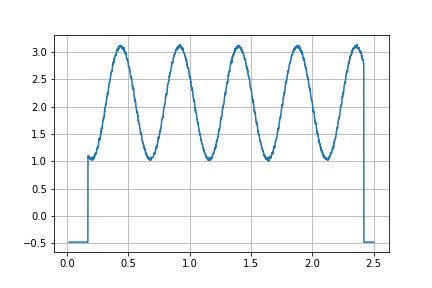
\includegraphics[width=12cm]{v4ori.png}
	\caption{Erzeugte Sinusschwingung durch DA-Wandlung}
\end{figure}

\begin{figure}[H]
	\centering\small
	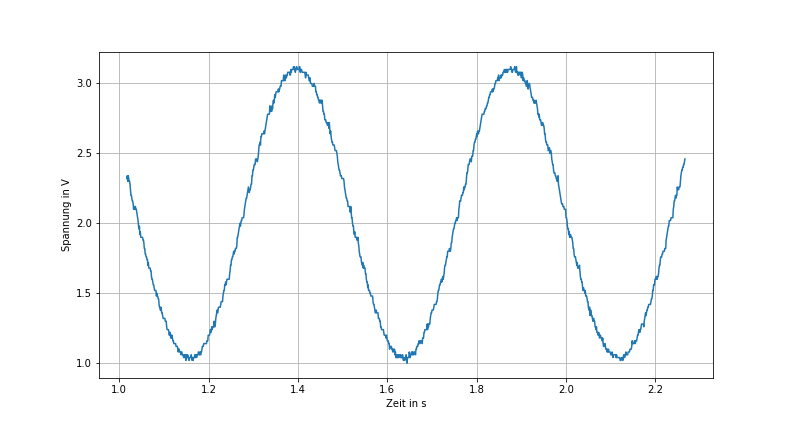
\includegraphics[width=15cm]{v4neu.png}
	\caption{Abgeschnittene und vergrößerte Sinusschwingung}
\end{figure}


\section{Auswertung}

\label{chap:VERSUCH_4_AUSWERTUNG}

\qquad Wir haben das Programm modifiziert, dass zwischen den einzelnen Ausgaben keine Pausen entstehen sollten, um die Wirkung von der Pause auf die Samplingrate zu analysieren.

\begin{figure}[H]
	\centering\small
	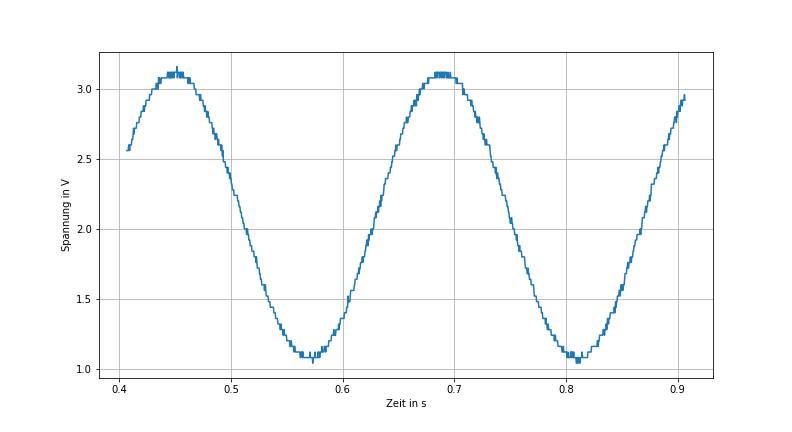
\includegraphics[width=15cm]{v4ohne.png}
	\caption{Erzeugte Sinusschwingung ohne Pause}
\end{figure}

Deutlich liefert es eine Sinusschwingung mit der größeren Frequenz als die von der mit Pause. Und die ohne Pause Schwingung hat mehr eckige Stelle in seiner Form(geringere Genauigkeit, da die Samplingrate von DA-Wandler nicht groß genug ist).


\section{Interpretation}
\label{chap:VERSUCH_4_INTERPRETATION}
\qquad Allgemein sehen die beide Sinusspannung ähnlich wie eine tatsächliche Sinusschwingung aus. Der Unterschied liegt daran, dass das Signal bei der Umwandlung von Digital in Analog nie kontinuierlich richtig dargestellt wird. 



%
% CHAPTER Versuch 5
%
\chapter{Abtasttheorem}
\section{Fragestellung, Messprinzip, Aufbau, Messmittel}
\qquad In diesem Versuch wird die tatsächliche Abtastfrequenz des AD-Wandlers ermittelt. Dazu soll ein Abtastfrequenz im Intervall[6000,8000] ausgewählt und mit dem entsprechenden RedLab-Befehl an den AD-Wandler gegeben werden. Dazu wird auch die Nyquist-Frequenz bestimmt.

Mit dem Sinusgenerator wird die Frequenz in 7 Schritten(angefangen von der halben Nyquist-Frequenz bis zur doppelten Nyquist-Frequenz) variiert und die Kurven davon grafisch darzustellen.

Den Code davon bitte den Anhang A.1.3.
\section{Messwerte}
\label{chap:VERSUCH_5_MESSWERTE}

\begin{figure}[H]
	\centering\small
	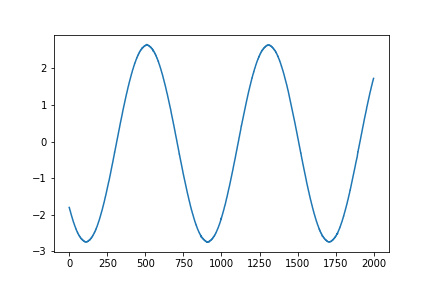
\includegraphics[width=12cm]{10.png}
	\caption{Schwingung mit der Frequenz 10Hz}
\end{figure}

\begin{figure}[H]
	\centering\small
	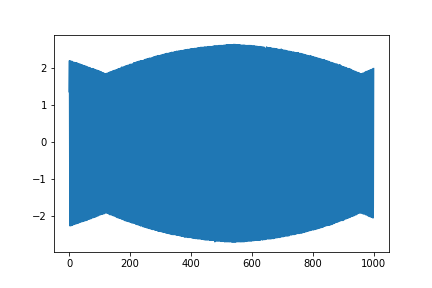
\includegraphics[width=12cm]{2000.png}
	\caption{Schwingung mit der Frequenz 2000Hz}
\end{figure}

\begin{figure}[H]
	\centering\small
	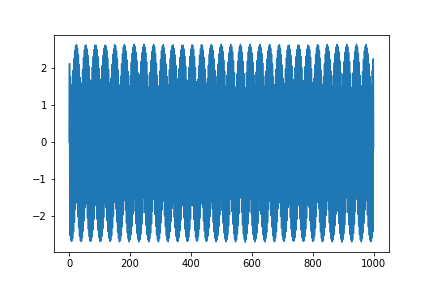
\includegraphics[width=12cm]{2750.png}
	\caption{Schwingung mit der Frequenz 2750Hz}
\end{figure}

\begin{figure}[H]
	\centering\small
	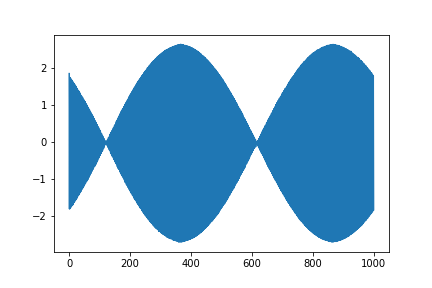
\includegraphics[width=12cm]{4000.png}
	\caption{Schwingung mit der Nyquist-Frequenz 4000Hz}
\end{figure}


\begin{figure}[H]
	\centering\small
	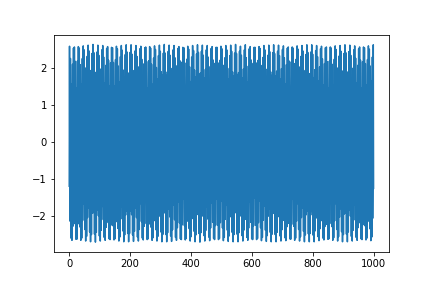
\includegraphics[width=12cm]{5500.png}
	\caption{Schwingung mit der Frequenz 5500Hz}
\end{figure}


\begin{figure}[H]
	\centering\small
	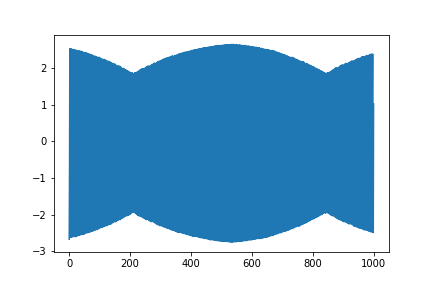
\includegraphics[width=12cm]{6000.png}
	\caption{Schwingung mit der Frequenz 6000Hz}
\end{figure}


\begin{figure}[H]
	\centering\small
	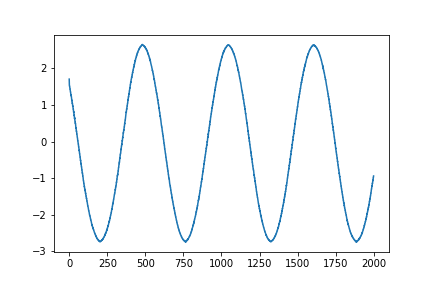
\includegraphics[width=12cm]{8000.png}
	\caption{Schwingung mit der Abtastfrequenz 8000Hz}
\end{figure}



\section{Auswertung}

\label{chap:VERSUCH_5_AUSWERTUNG}

\qquad Hierfür wurde 8000 Hz als Abtastfrequenz ausgewählt. Die tatsächliche Abtastfrequenz des AD-Wandlers beträgt 8021 Hz. Die Nyquist-Frequenz ist halbe Abtastfrequenz(4000 Hz).

\section{Interpretation}
\label{chap:VERSUCH_5_INTERPRETATION}
\qquad Nach dem Abtasttheorem sind die Sinusschwingungen mit der Frequenz unter Nyquist-Frequenz darstellbar. D.h. die Wellenform ist keine Sinusform mehr trotzdem bleibt die Frequenz erhalten. Eine Sinusschwingung mit der Frequenz höher als Nyquist-Frequenz aber kleiner als Abtastfrequenz wird nicht mehr fehlerfrei aus dem abgetasteten Signal rekonstruiert. Es wird so rekonstruiert als ob es eine Spiegelung an Nyquist-Frequenz stattfindet z.B. 6000 Hz(4000 Hz + 2000 Hz) ist die Spiegelung von 2000 Hz(4000 Hz - 2000 Hz). Deswegen sehen Abbildungen 5.2 und 5.6 / 5.1 und 5.7 fast gleichförmig aus.



%
% CHAPTER Anhang
%
\renewcommand\thesection{A.\arabic{section}}
\renewcommand\thesubsection{\thesection.\arabic{subsection}}

\chapter*{Anhang}
\label{chap:APPENDIX}
\addcontentsline{toc}{chapter}{Anhang}
%\setcounter{chapter}{0}
\addtocounter{chapter}{1}
\setcounter{section}{0}

\section{Quellcode}
\label{chap:APPENDIX_SOURCECODE}

\subsection{Quellcode Versuch 1-3}
\label{chap:APPENDIX_SOURCECODE_V1}
\begin{lstlisting}[
style=PYTHON,
frame=single,
caption=,
captionpos=b,
label=lst:V1]
import redlab as rl
import matplotlib.pyplot as pl

print("------- einzelne Werte -------------------------")
print("16 Bit Value: " + str(rl.cbAIn(0,0,1)))
print("Voltage Value: " + str(rl.cbVIn(0,0,1))) #Versuch2
print("------- Messreihe -------------------------")
a = rl.cbVInScan(0,0,0,1000,8000,1)
print("Messreihe: " + str(a))
pl.plot(a)
pl.show()
print("Messreihe: " + str(rl.cbVInScan(0,0,0,300,8000,1)))
print("Samplerate: " + str(rl.cbInScanRate(0,0,0,8000)))
###Konsoleneingaben### #versuch3
x = input("Spannung:")
x = float(x)
rl.cbVOut(0,0,101,x) 
\end{lstlisting}

\subsection{Quellcode Sinusschwingung-Generator Versuch4}
\label{chap:APPENDIX_SOURCECODE_V1}
\begin{lstlisting}[
style=PYTHON,
frame=single,
caption=,
captionpos=b,
label=lst:V4]
import redlab as rl
import numpy as np
import time
import matplotlib.pyplot as pl

x = np.linspace(0,2 * np.pi,30, endpoint=False)
print(np.sin(x))
while(1):
    for i in x:
        rl.cbVOut(0,0,101,np.sin(i)+2)
        time.sleep(0.01)
        
####für Darstellung###
#v4 = np.genfromtxt("v4_Messwert.csv",delimiter=",",skip_header=17)
#x = v4[1000:2250,3:4]
#y = v4[1000:2250,4:5]
#pl.figure(figsize=(11,6))
#pl.xlabel('Zeit in s')
#pl.ylabel('Spannung in V')
#pl.plot(x,y)
#pl.grid()
#pl.savefig('v4neu.png')
#pl.show()
\end{lstlisting}

\subsection{Quellcode Versuch 5}
\label{chap:APPENDIX_SOURCECODE_V2}
\begin{lstlisting}[
style=PYTHON,
frame=single,
caption=,
captionpos=b,
label=lst:V5]
import redlab as rl
import numpy as np
import matplotlib.pyplot as pl

print("Samplerate: " + str(rl.cbInScanRate(0,0,0,8000)))
a = rl.cbVInScan(0,0,0,1000,8000,1)
np.save('5500Hz', a)

index = [10,2000,2750,4000,5500,6000,8000]


for i in index:
    v5 = np.load(str(i)+'Hz.npy')
    pl.plot(v5)
    pl.savefig(str(i) + '.png')
    pl.show()
    
\end{lstlisting}
\end{document}
%------------------------------------
% ╔═╗╔╗╔╔╦╗  ╔╦╗╔═╗╔═╗╦  ╦╔╦╗╔═╗╔╗╔╔╦╗
% ║╣  ║║║  ║║     ║║║  ║║    ║  ║║║║║ ╣  ║║║ ║ 
% ╚═╝╝╚╝═╩╝  ═╩╝╚═╝╚═╝╚═╝╩  ╩╚═╝╝╚╝  ╩ 
%------------------------------------